\chapter{Background}
This chapter aims to provide all the required background knowledge to understand the concepts discussed in the report. The contribution of the report involves extending a concurrent, message-passing language to be verification-aware. We define a verification-aware language as a language that strongly couples specifications and implementations. To understand how this can be done with a message-passing language, we must first form strong fundamentals in concurrency and existing verification techniques.
\\ \\
We start by introducing core concurrency concepts in section \ref{sec:concurrency}. We will explore memory models, safety, liveness and fairness. Section \ref{sec:model_checking} will introduce model checking and compare some of the existing state-of-the-art model checkers. Finally, we will discuss what a verification-aware language is and why they are important to modern system design in \ref{sec:existing_work}
\section{Concurrency} \label{sec:concurrency}
Concurrency introduces a notion for multiple components of a program to execute out-of-order. We saw in the previous section how multiple processes can be composed and treated as a single execution. For example, given two processes with disjoint alphabets, the parallel composition can result in any interleaving. This section aims to explore further in-depth the principles of concurrency, moving away from a mathematical representation and looking at higher-level concepts such as consistency models and temporal logic. 
\\ \\
Concurrency is a core concept in classical distributed algorithms, such as the Paxos algorithm \cite{basic_paxos}, Raft \cite{raft} and Dining Philosophers \cite{dining_philosophers}. The capability for concurrency has grown with better hardware. Concurrency introduces the idea of consistency models \cite{art_of_multiprocessor_programming} to help reason about executions of multi-threaded systems. Lamport introduced sequential consistency \cite{sc} as a strong safety property for concurrent systems. Sequential consistency can be informally reasoned about by considering a single-core processor: if multiple threads are executed in parallel on a single-core processor, only one instruction can be executed at a time. This means that the result of any execution forms a total order, consistent with the order of operations on each individual process. For example, consider a new composition where a sequence of events has been executed by a teacher, \((teach \rightarrow teach \rightarrow)\), and a student is scheduled to execute next. Under the sequential consistency model the student must observe the same order of events as the teacher.
\\ \\
Weaker memory models exist, which allow us to model systems that do not guarantee sequential consistency (for example, systems running on multi-core processors). Under these models, the instructions of a thread may be reordered (i.e. execute out-of-order) which introduces weak behaviours that we would not observe under sequential consistency. For example, total store ordering is a weaker memory model, that allows the reordering of write-read operations on different memory locations within a single thread. For the examples discussed in this report, we will assume a sequentially consistent model.

\subsection{The Actor Model}
The actor model \cite{actors} is a model of concurrent computation that treats actors as primitive components of the system. A concurrently executed actor is defined in terms of three key behaviours.
\begin{itemize}
    \item An actor can send a number of messages to other actors
    \item An actor can create a a number of new actors
    \item An actor can act in response to a message it receives
\end{itemize}
Tony Hoare introduced Communicating Sequential Processes (CSP), a mathematical notation for defining processes and interactive systems \cite{csp_paper}. CSP provides a framework for reasoning about the behaviour of concurrent systems which has influenced distributed algorithms \cite{distributed_algorithms_na_lynch}, model checking \cite{model_checking} and many other related research fields.
\\ \\
The CSP model uses channels to communicate between actors. A channel is a communication medium that allows processes to send and receive messages. Under this model, an actor can output a value $v$ on a channel $c$, using the ! operator.
\[
c!v
\]
Similarly, an actor can input a value $x$ on a channel $c$ using the ? operator.
\[
c?x
\]
The concept of channels has been used in modern programming languages, such as Go \cite{go}, as well as verification modelling languages like Promela \cite{promela}. Akin to channels, we introduce mailboxes. Under a mailbox model, an actor has a designated mailbox, where messages are stored. An actor can read messages from its mailbox and act upon them. For example, Elixir \cite{elixir}, handles all communication through process owned mailboxes. Channels and mailboxes give us an alternative model to that of shared memory.
\\ \\
In a shared memory model, a shared memory region is established in which multiple processes can read and write. Figure \ref{fig:shared_memory} shows a basic example of two processes that write to a shared in-memory array. Due to how often we see shared memory used in large-scale distributed systems, much work has been done in the verification of these systems using shared memory models. For example, Jon Mediero Iturrioz used Dafny \cite{dafny} to prove the correctness of concurrent programs that implement shared memory \cite{shared_memory_verification}. 
\begin{figure}[h]
    \centering
    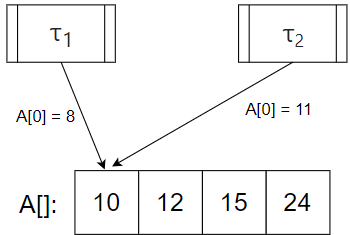
\includegraphics[width=0.4\textwidth]{images/shared_memory.png}
    \caption{An example of two processes writing to a shared in-memory array}
    \label{fig:shared_memory}
\end{figure}
\\ \\
By contrast, figure \ref{fig:actor_model} shows an example of how actors behave using mailboxes. The mailbox is not necessarily first in, first out (FIFO) but often implementations tend to be.
\begin{figure}[H]
    \centering
    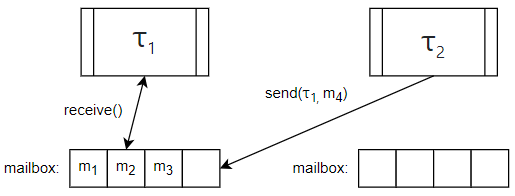
\includegraphics[width=0.6\textwidth]{images/actor_model.png}
    \caption{An example of actors sending and receiving messages under the actor model}
    \label{fig:actor_model}
\end{figure}
\subsection{Temporal Logic}
First-order logic, or predicate logic uses quantifiers to reason about the truth of statements. For example, the statement $(\forall x \in \mathbb{N} \,.\, x > 0)$ is true for all natural numbers $\mathbb{N}$, and uses the universal quantifier $\forall$, to quantify over all x. We can also use the existential quantifier $\exists$, to reason about the existence of an element in a set. First-order logic is a powerful tool for reasoning about the truth of statements, but it cannot reason about time and change. We introduce modal logic for this purpose.
\begin{bnf*}
    \bnfprod{A}
      {p \bnfor \top \bnfor \neg \bnfpn{A} \bnfor \bnfpn{A} \land \bnfpn{A} \bnfor \square \bnfpn{A}}\\
\end{bnf*}
Where A is a modal formula, $p$ is an atomic proposition, $\top$ represents `truth' and $\square A$ reads box A. Using rules from first-order logic we can introduce disjunct, implication and if-and-only-if. We can also introduce the second modal operator, $\lozenge A$ which reads diamond A.
\[
\lozenge \langle A \rangle \models \neg \square \neg \langle A \rangle
\]
Depending on the circumstances that box and diamond are applied, they have different readings. For example, in temporal logic, $\square A$ can read as `always A' and $\lozenge A$ can read as `sometimes A', informally, it can be useful to think of $\square$ similarly to $\forall$ and $\lozenge$ to $\exists$.
\\ \\
Saul Kripke introduced Kripke semantics \cite{kripke} for reasoning about temporal logic. For example, consider modelling a system based on our student and teacher processes. We let $M$ be the model of the system and $s$ represent a singular state the system can be in. Typically, $s$ is the initial state of the system. If we are given a temporal formula $A$, we can now define the syntax for the truth of $A$ in state $s$ of the model $M$.
\[
(M, s) \models A
\]
To reason formally about what it means for $A$ to hold in state $s$, Kripke provided formal definitions for the base and inductive definitions of $A$.
\\ \\
We finally extend this understanding of temporal logic to linear temporal logic (LTL), or sometimes written as linear-time temporal logic. LTL allows us to reason about the time and change of a model. Before we provide some examples, we introduce a final temporal operator, $U$, which reads until. The formula $\phi U \psi$ defines the truth of $\phi$ until $\psi$ holds. We call this `strong until' as there must exist a state where $\psi$ becomes true. `Weak until' $W$, can also be defined, which loosens the restrictions such that $\phi$ could hold for the entire execution.
\\ \\
We can now explore a few basic examples of LTL formulas as well as provide some intuition behind them. We define a set of atomic propositions, $AP = \{study, sleep, tired, exam\}$.
\begin{multicols}{2}
    \[
    \begin{aligned}
    &\square \ \text{sleep} \\
    &\text{tired} \, U \, \text{sleep} \\
    &\square (\text{study} \Rightarrow \text{tired}) \\
    &\square \ \text{study} \Rightarrow \lozenge \ \text{exam}
    \end{aligned}
    \]
    \vline
    \[
    \begin{aligned}
    \text{Always sleeping} \\
    \text{Tired until sleeping} \\
    \text{Studying implies always tired} \\
    \text{Always studying implies eventually an exam}
    \end{aligned}
    \]
    \end{multicols}
Alongside LTL, other forms of temporal logic exist, such as Computation Tree Logic (CTL) \cite{temporal_and_modal_logic} and Alternating-time Temporal Logic (ATL) \cite{atl}. CTL introduces path quantifiers to reason about specific traces through a model, and ATL introduces the idea of agents, where agents can work in coalitions to achieve a goal in the system. Temporal logic is an important concept in the model checking of systems \cite{principles_of_model_checking}, see chapter \ref{sec:model_checking}. 
\subsection{Safety and Liveness}
Safety and liveness are properties that can be specified about systems. A safety property can be intuitively thought of as a property such that nothing bad happens, and a liveness property is where something good will happen. For example, something bad could be a deadlock in a system, and something good could be that the system will eventually reach a consensus. We define safety informally as: given a finite execution $E$ and a state $s$ such that $s$ is the final state in the execution, we can say that a safety property $P$ holds if $P$ is true in $s$ and all previous states in $E$. If $s$ violates $P$, then $E$ violates $P$. Unlike with safety, we cannot determine the truth of a liveness property at $s$, we must instead inspect an infinite execution $E'$. We express these properties as temporal formulas. For example, we can specify a simple liveness property to ensure our student will always study again.
\[
\square \lozenge \text{study}
\]
To help understand why this is a liveness property, consider two states, $s_1$ and $s_2$. Take the assignment of $study$ to be $\{s_1\}$ i.e., $study$ is true only in $s_1$. Regardless of if we want to reason about the truth of the formula at $s_1$ or $s_2$, we cannot, as the box operator requires the formula to hold in all states. Hence, we would have to inspect the current state, as well as an infinite future execution from the state, to determine the truth of the formula. Because no single state exists where we can evaluate the truth of the formula, we can convince ourselves it is a liveness property.
\\ \\
We use the same assignment of study to reason about a new property.
\[
\square \ \text{study}
\]
We can understand intuitively why this property is a safety property by considering $s_2$. As $s_2$ is not in the assignment of study (i.e. $study$ is false in $s_2$), any execution that passes through $s_2$ will violate the property. As we can determine the truth of the property with a finite execution, we can deem the property a safety property.
\\ \\
By using both safety and liveness properties, we can define a `correct' system, through the evaluation of these temporal formulae.
\subsection{Fairness}
Fairness introduces more properties that can be defined using temporal formulae. Fairness properties do not target the specification of the system in the same way that other properties we have looked at do. Instead, fairness properties are constraints on the scheduling of the system. They aim to fairly select which process to execute next. Without fairness, a system could favour the scheduling of process A while never progressing with process B. We will discuss two flavours of fairness, weak fairness and strong fairness. Properties that hold under weak fairness also hold under strong fairness, hence strong implies weak. To define the fairness properties, we must first define what it means for an event to be enabled. An event (or action) $A$ of a process algebra is enabled if it can be executed in the current state. We will use the notation $A_E$ to denote an enabled event, for example, $study_E$ denotes the study event is executable in the current state. We now define weak fairness (WF) and strong fairness (SF).
\[
\begin{aligned}
&WF \, A \equiv \lozenge \square A_E \Rightarrow \square \lozenge A \\
&SF \, A \equiv \square \lozenge A_E \Rightarrow \square \lozenge A \\
\end{aligned}
\]
We can informally define weak fairness as: if an event is continuously enabled, it is executed infinitely often. Similarly, strong fairness reads: if an event is repeatedly enabled, it is executed infinitely often.
\section{Model Checking} \label{sec:model_checking}
Model checking is the process of determining if a finite-state machine (FSM) is correct under a provided specification. It typically involves enumerating all possible states of an FSM and ensuring the correctness of each state. For example, given a model M and a property $\varphi$, if no state of M violates $\varphi$, then we can say M satisfies $\varphi$. In software development, model checkers are beneficial in providing guarantees for safety-critical systems as well as concurrent systems. Concurrent systems can often cause issues with uncommon instruction execution interleaving that are not easily identifiable until long into a runtime. For example, deadlocks can occur when instructions being run by two processes are dependent on one another making progress. A simple example of a deadlock that can occur, is the following interleaving of instructions executed by two processes, $\tau_1$ and $\tau_2$. 
\begin{multicols}{2}
    \[
    \begin{aligned}
    & \tau_1: \text{ acquire lock A} \\
    & \tau_1: \text{ acquire lock B} \\
    & \tau_1: \text{ release locks}
    \end{aligned}
    \]
    \vline
    \[
    \begin{aligned}
    & \tau_2: \text{ acquire lock B} \\
    & \tau_2: \text{ acquire lock A} \\
    & \tau_2: \text{ release locks}
    \end{aligned}
    \]
    \end{multicols}
An interleaving such as ($\tau_1$, $\tau_2$, $\tau_1$, $\tau_2$, \dots) results in $\tau_1$ blocking until it can acquire lock B, and $\tau_2$ blocking until it can acquire lock A, hence the program is in a deadlock. Due to the nature of concurrent systems, we could run our program and never experience this interleaving of instructions from occurring, hence we could deem our program deadlock-free. Instead, by abstracting our program as a model, and verifying the correctness using a model checker, we could exhaustively check all possible states (interleaving of concurrent processes) and catch this deadlock. 
\\ \\
Alongside determining progress can be made within a system, model checkers are also used to guarantee the correctness of a specification. To demonstrate, we model a very simple 24-hour clock, where at each time step, we progress time by an hour.
\[
\begin{aligned}
& \tau_1: \text{time} \leftarrow \text{time} + 1
\end{aligned}
\]
Unlike the previous example, this process can always make progress so will not result in a deadlock, however, it is not a correct implementation of a 24-hour clock. We would like our 24-hour clock to only represent times in the range 1 to 24. By introducing a specification alongside our model, we can use a model checker to determine if all the states of our program adhere to the specification. In this instance, we would just need to specify a bound over our time variable.
\[
\{ \text{time} \mid \text{time} \in \mathbb{N}, 1 \leq \text{time} \leq 24 \}
\]
This is a simple example of a specification, that we can write in a specification language and use in tandem with our model to check the correctness of using a model checker. For a given model $M$ and a property $\phi$, we formally define model checking as the process of computing if $M \models \phi$ (satisfiability).
\subsection{A Comparison Of Model Checkers}
Many model checkers have been invented for this reason, each with different focuses and specification languages. This section will comment on some of the more common model checkers and discuss their functionalities. We first provide an overview of the capabilities and limitations of many model checkers, before providing a more in-depth look into model checkers best aligned with the goals of this report.
\\ \\
\subsubsection{Overview}

\begin{table}[ht]
    \centering
    \begin{tabular}{|>{\raggedright\arraybackslash}p{3cm}|
        >{\centering\arraybackslash}p{2cm}|
        >{\centering\arraybackslash}p{2cm}|
        >{\centering\arraybackslash}p{3cm}|
        >{\centering\arraybackslash}p{3cm}|}
        \hline
        \textbf{Model Checker} & \textbf{LTL Support} & \textbf{CTL Support} & \textbf{Probabilistic} & \textbf{Concurrency Support} \\
        \hline
        PAT & Yes & No & Yes & Yes \\
        \hline
        BLAST & No & No & No & Limited \\
        \hline
        SPIN & Yes & No & No & Yes \\
        \hline
        TLC & Yes & No & No & Yes \\
        \hline
        PRISM & Yes & Yes & Yes & Yes \\
        \hline
        NuSMV & Yes & Yes & No & Yes \\
        \hline
        UPPAAL & No & No & Yes & Yes \\
        \hline
    \end{tabular}
    \caption{Comparison of Model Checkers}
    \end{table}
\subsubsection*{\textbf{PAT}}
Process Analysis Toolkit (PAT) is a self-contained framework to support composing, simulating and reasoning of concurrent, real-time systems \cite{pat}. PAT is based on Tony Hoare's CSP and extends the language using its library called CSP\#. CSP\# is a superset language of the original CSP, hence all classical CSP models can be verified with PAT. PAT has shown to be capable of verifying classical concurrent algorithms such as the dining philosophers problem. Alongside its verification capabilities, the PAT toolkit can be used to simulate real-world scenarios over specifications. 
\\ \\
PAT's ability to determine the correctness of classical process algebra means it is a strong, widely applicable model checker.

\subsubsection*{\textbf{BLAST}}
BLAST is an automatic verification tool for checking the temporal safety properties of C programs. Given a C program and a temporal safety property, BLAST either statically proves the program satisfies the property or provides an execution path that exhibits a violation of the property \cite{blast}.
\\ \\
Where BLAST differs from PAT, is that it no longer relies on process algebra. The model checker is capable of running directly on a subset of C programs where no intermediate modelling is required. As an end-user tool, this is more generally applicable than PAT; there is no burden on developers to think about how to model their systems with process algebra and instead can directly get safety guarantees from their programs. BLAST handles the translation of C programs to an abstract reachability tree (ART), a labelled tree that represents a portion of the reachable state space of the program. Using a context-free reachability algorithm on this representation of a C program, means temporal properties can be checked, without the end programmer being required to think about what the control-flow automata for the program will look like.
\\ \\
BLAST falls short when model-checking large C programs. More importantly, it is unable to provide any guarantees on concurrent programs. We are primarily concerned with concurrent systems in this report, as Elixir is a language that is designed for building concurrent systems.

\subsubsection*{\textbf{PRISM}}
PRISM is a probabilistic model checker, a tool for formal modelling and analysis of systems that exhibit random behaviour or probabilistic behaviour \cite{prism}. It has been used to analyse systems implementing randomised distributed algorithms.

\subsubsection*{\textbf{TLC}}
In 1980, Leslie Lamport formulated the Temporal Logic of Action (TLA) \cite{tla}. TLA is a logic system for specifying and reasoning about concurrent systems. Both the systems and their properties are represented in the same logic, so that the assertion that a system meets its specification, can be expressed by a logical implication.
\\ \\
TLA is capable of specifying complex systems but in a typically verbose manner. Leslie Lamport introduced TLA+ \cite{tlaplus}, combining mathematical ideas with concepts from programming languages to create a specification language that would allow mathematicians to write specifications in 20 lines as opposed to 20 pages.
\\ \\
Furthering on from Leslie Lamport's discovery of these specification languages, Lamport created TLC \cite{tlc}, a model checker for the verification of TLA+ specifications. Similarly to BLAST, TLC builds a finite-state machine from the specification so the model checker can verify and debug invariance properties over it. TLC has been used to verify many large-scale, real-world systems specified in TLA+. Not only does it verify temporal properties of TLA+ specifications, but it can also model check PlusCal \cite{pluscal} algorithms. PlusCal is an algorithm language aimed to resemble that of pseudocode, but PlusCal algorithms can be automatically translated to TLA+ specifications to be reasoned about formally with TLC. We have already come across the concept of model-checking algorithms as opposed to specifications with BLAST, but instead of being strictly bound to the C programming language, PlusCal provides a more general framework agnostic of a choice of programming language allowing developers to separate reasoning about algorithms from their respective programs.

\subsubsection*{\textbf{SPIN}}
Spin is an efficient verification system for models of distributed software systems. It has been used to detect design errors in applications ranging from high-level descriptions of distributed algorithms to detailed code \cite{spin}. Spin has a specification language, Process Meta Language (Promela), which the model checker uses to prove the correctness of asynchronous process interactions. Spin supports asynchronous process communication through channels, where processes can send and receive messages. Spin constructs labelled transition systems for respective processes from Promela specifications, which it goes on to use for scheduling and to reason about properties of the model. Because many programming languages, such as GO \cite{go} rely on the creation of channels for asynchronous communication between processes, Promela becomes a natural solution to modelling these systems.
\subsubsection{Summary}
We have discussed a selection of model-checkers and what their primary focus is. Many existing model-checkers have been originally designed to prove specifications over sequential models. Some have taken this further and applied model checking directly over programming languages, such as BLAST. Other model-checkers have introduced some primitives for reasoning about concurrency. TLC allows for the specification of processes and using structures can begin to specify shared memory. Similarly, Spin allows processes to be specified and supports the creation of channels for communication. Despite this, none of the model checkers discussed, include message-passing as a first-class construct. To reason about message-passing models, such as the actor model, work has to be done to formalise actor-based constructs. This makes specifying actor-based systems, such as systems written in Elixir, a non-trivial task.

\section{Related Work} \label{sec:existing_work}
Much work has gone into model checking, theorem-proving and verifying the implementations of systems. For Elixir, there are tools such as dialyzer \cite{dialyzer}, which statically analyse Elixir programs for type errors or dead code. Whilst these tools provide Elixir developers better guarantees, it does not verify the correctness of a system as a whole. Elixir also has libraries for property-based testing, such as PropEr \cite{proper}, which can be used to generate random test cases for a system. Property-based testing randomly generates inputs to test a system, which can be useful for finding edge cases that unit tests may not cover. However, property-based testing does not provide guarantees about the correctness of a system, instead, it is used to find bugs in code. Work has also gone into verifying message-passing in Elixir, using binary session types \cite{binary_session_types}. This approach ensures two processes, communicating over compatible protocols, avoid certain communication errors (i.e. hanging messages), but has not been extended to multiparty session types, so is not appropriate for verifying all actor-based systems.
\\ \\
There is also existing work in the greater verification of real-world software. Much of this is done on sequentially executed programs as concurrency introduces a new level of complexity. For example, both C programs and GO programs have previously been targetted as good options for model checking \cite{gomela, c_to_promela}. While these tools provide system guarantees, they primarily focus on detecting deadlocks or dataraces within a system and do not support other safety or liveness properties.
\subsection{Theorem Proving}
Theorem proving takes a formal approach to program verification. In theorem proving, axioms are applied to a set of statements to determine if a particular statement holds. For example, Z3 \cite{z3} is a satisfiability modulo theories (SMT) solver developed by Microsoft that can verify propositional logic assertions.
\subsection{Design by Contract}
Design by Contract (DbC) is an approach to software design, where software components are defined using formal specifications \cite{dbc}. A contract is composed of three elements.
\begin{itemize}
    \item \textbf{Pre-condition}: A condition that must be true before a function is executed.
    \item \textbf{Post-condition}: A condition that must be true after a function is executed.
    \item \textbf{Invariant}: A condition that must be true before and after a function is executed.
\end{itemize}
These properties are known as assertions. Some programming languages directly support assertions, such as Eiffel \cite{eiffel}. When formalising a contract, an agreement is established between two parties, the client and the contractor. The client is entitled to receive a result that satisfies the post-condition. Similarly, the contractor is protected by the pre-condition, such that, no unintended behaviour occurs.
\\ \\
Design by contract is a contribution to software reliability. In modern languages, the client and contractor are often functions or methods, which call one another. Verification-aware languages such as Dafny \cite{dafny_paper} support the specification of contracts, on methods, which can be verified.
\subsection{Verification-aware Languages}
Verification-aware languages are a new trend in programming languages, where the language is designed to support proving the correctness of a program. Examples of these include Lean, Dafny and Boogie. We will explore some of these languages in detail to understand how verification-aware languages can be a powerful tool to reason about the correctness of a system. The conventional alternatives involve either disregarding formal methods entirely or hand translating a program into a specification language, such as TLA+. A good verification-aware language should naturally integrate the system specification with the implementation. The aim is to reduce the burden on programmers to maintain separate specifications alongside evolving codebases.
\subsubsection{Lean}
The Lean theorem prover is a proof assistant developed by Leonardo de Moura \cite{lean}. Lean is first and foremost, a functional programming language, designed to write correct and maintainable code. Lean can be used as an interactive theorem prover, where developers can write proofs alongside code. It supports many features of modern-day functional languages, such as first-class functions, pattern matching and even multithreading. A proof assistant is a language that allows developers to define objects and specifications over them. They can be used to verify the correctness of programs (similar to a model checker) as they check proofs are correct using logical foundations. The theorem proofs typically involve solving constraint problems, by determining if a first-order formula can be satisfied concerning constraints generated during analysis of functions.
\\ \\
While Lean is itself both a functional programming language and theorem prover, this approach differs in implementation from other theorem provers, such as Dafny, which instead prove theorems using existing backend theorem provers.

\subsubsection{Dafny}
Dafny is a verification-aware programming language that has native support for inlining specifications that can be verified by a theorem prover \cite{dafny_paper}. Dafny aims to modernise the approach developers take to designing systems, by encouraging developers to write correct specifications. With the rise of modern theorem provers, this untraditional approach is now realistic. Dafny is an imperative language with methods, variables, loops and many other features of typical imperative programming languages. Dafny programs are equipped with supporting tools to translate to other imperative languages, such as Java and Python. 
\\ \\
Dafny verifies the correctness of programs using the theorem prover, Z3 \cite{z3}. Developers can write specifications alongside code, such as methods, which can then be directly verified. The format of specifications typically follows those of a Hoare Triple, $\{P\}C\{Q\}$, such that given a precondition, $\{P\}$ holds, if $C$ terminates, a post-condition, $\{Q\}$, will hold. In Dafny, the language reserves the keywords \texttt{requires} and \texttt{ensures} for pre and post-conditions. Listing \ref{fig:dafny_add} shows a basic example of a Dafny method, which introduces an \texttt{Add} method. The implementation unintentionally introduces a bug such that, any execution paths with an input $\{ a \in \mathbb{Z} \mid a < 0 \}$ do not necessarily return the sum of the two inputs. Because Dafny places the burden on writing good specifications as opposed to correct code, the underlying theorem prover can use our post-condition to flag that this program is not correct for all execution paths.
\begin{lstlisting}[language=Dafny, xleftmargin=.3\linewidth, caption={Example of a method in Dafny}., label={fig:dafny_add}]
    method Add(a: int, b: int) returns (c: int)
        ensures c == a + b;
    {
        if  a < 0 {
            c := -1;
        } else {
            c := a + b;
        }
    }
\end{lstlisting}
Listing \ref{fig:dafny_add} only gives a small insight into the power the Dafny specification language defines. Alongside the evaluation of basic expressions, Dafny allows the use of quantifiers such as the universal quantifier. The introduction of quantifiers, allows us to write pre- and post-conditions over collections of objects, such as sets and arrays. Listing \ref{fig:dafny_quantifier} shows a basic example of how the universal quantifier can be used with the underlying theorem prover, to assert all the elements of an array, \texttt{a[]}, are strictly positive.
\begin{lstlisting}[language=Dafny, numbers=none, xleftmargin=.3\linewidth, caption={\texttt{forall} quantifier in Dafny \cite{dafny_tutorial}}., label={fig:dafny_quantifier}]
forall k: int :: 0 <= k < a.Length ==> 0 < a[k]
\end{lstlisting}
Dafny also uses other concepts that support the verification of programs. Assertions can be used to provide guarantees in the middle of a method. Loop invariants can annotate while loops to check a condition holds, upon entering a loop and after every execution of the loop body. Similarly, loop variants can be used to determine termination of while loops, by checking that every execution of a loop body makes progress towards the bound of the loop.
\subsubsection{Boogie}
Boogie is a modelling language intended as an intermediate verification language (IVL), developed at Microsoft \cite{boogie}. The language is described as an intermediate language because it is designed to bridge the gap between a program and a program verifier. Many tools that rely on Boogie's intermediate representation, are doing so to translate source code in a native language into a format that can be proved. Dafny is a prime example of a programming language which does so. The Dafny compiler generates Boogie programs that can then be verified by Z3. This provides multiple benefits for Dafny. Firstly, Dafny does not have to concern itself with being dependent on a specific SMT solver, such as Z3. Instead, it can be designed agnostic to the choice of theorem prover, as Boogie will take responsibility for handling interaction with theorem provers. Boogie also bears a closer resemblance to an imperative programming language (like Dafny), so translation between the two is easier than translating to Z3. Listing \ref{fig:boogie_add} shows an example Boogie program, defining a single procedure, \texttt{add}, that represents the translated code from the Dafny example in listing \ref{fig:dafny_add}. Note the similarities between both programming languages, both use \texttt{ensures} to capture preconditions and have very similar syntax and control flow. However, now that our program is written in the Boogie IVL, we can directly determine an execution path that violates the precondition using a theorem prover such as Z3.
\begin{lstlisting}[language=boogie, xleftmargin=.3\linewidth, caption={An example Boogie IVL program}., label={fig:boogie_add}]
procedure add(a: int, b: int) returns (c: int)
    ensures c == a + b;
{
    if (a < 0) 
    {
        c := -1;
    } else {
        c := a + b;
    }
}
\end{lstlisting}

\subsection{Deadlock Detection}
Alongside research into verification-aware languages, there has been work into detecting deadlocks in concurrent systems. These approaches typically involve the use of model checkers to determine if a system can reach a deadlock state. For example, Java Pathfinder \cite{jpf} is a model checker for Java programs. It can be used to detect deadlocks and data races. The initial version of Java Pathfinder was a translator from Java to Promela. Since, Java Pathfinder now uses a Java Virtual Machine (JVM) implementation directly to model check Java programs.
\\ \\
There has also been work into detecting deadlocks in GO programs. Gomela \cite{gomela} was proven to catch more deadlocks than GCatch \cite{gcatch} and Godel2 \cite{godel2}. Gomela focuses on channeled communication between goroutines. Similarly, deadlock detection has been researched for C programs \cite{c_to_promela}. 
\\ \\
None of these approaches capture the semantics involved in a pure message-based, actor model. They also do not provide guarantees about the liveness properties of a system. This is a limitation in existing research of verification tools concerning modern programming languages.
\section{Summary}
This chapter has provided an overview of core concepts related to concurrent programs and verification of them. We saw process algebra that can be used to model and reason about concurrent processes, as well as Hoare Logic and its definition of the Hoare Triple as a fundamental property in verification. We also looked at applications based on this theory, such as model checkers, theorem provers and programming languages. Much work relating to the topic of verifying programming languages was explored, but importantly, we learned about SPIN. We also learned about Boogie, the intermediate verification language that can verify programmatic assumptions using Z3. This chapter also discussed some of the limitations in existing research, such as a need for new techniques to verify the liveness properties of real-world systems. The next chapter will discuss the Elixir programming language.

